\documentclass[aspectratio=169,10pt]{beamer}

% ---------------------------------------------------------------------------
% TP5 - EXPERIMENTOS EXTRA (borrador para discutir con el equipo).
% Mismo tema que la presentacion principal (Metropolis), en espanol.
% Figuras generadas por los scripts de extra/ (ver extra/*.py).
% Compilar: pdflatex main.tex  (x2)
% ---------------------------------------------------------------------------

\usetheme{metropolis}
\usepackage[utf8]{inputenc}
\usepackage[T1]{fontenc}
\usepackage[spanish]{babel}
\usepackage{graphicx}
\usepackage{booktabs}
\usepackage{amsmath}
\usepackage{xcolor}

\graphicspath{{../extra/results/}}

\title{TP5 --- Experimentos extra}
\subtitle{Borrador para discusion: ¿cuales integramos a la presentacion principal?}
\author{Sistemas de Inteligencia Artificial --- ITBA}
\date{}

\begin{document}

\maketitle

\begin{frame}{De que se trata este anexo}
  Cuatro experimentos \textbf{adicionales} (numpy puro, reusando el VAE ya
  gradchequeado del EJ2). No estan en la presentacion principal; la idea es
  verlos y decidir cuales valen la pena.
  \begin{itemize}
    \item \textbf{A --- VAE sobre el dataset del EJ1 (las letras).} Puente
          AE$\to$VAE sobre los \emph{mismos} datos: ¿que aporta el VAE?
    \item \textbf{B --- Unidades activas / posterior collapse.} \emph{Por que}
          satura el barrido de dimension latente (16--32).
    \item \textbf{D --- Generalizacion (split train/test).} ¿El VAE de emojis
          memoriza o generaliza? (disciplina del TP3, hoy ausente en EJ2).
    \item \textbf{E --- MSE vs BCE.} El clasico ``MSE borroso, BCE nitido''.
  \end{itemize}
  \vfill
  {\footnotesize Todo reproducible: \texttt{python3 extra/\{vae\_letters,active\_units,generalization,recon\_loss\}.py}.}
\end{frame}

% ===========================================================================
\section{A --- VAE sobre el dataset del EJ1 (letras)}

\begin{frame}{El VAE sobre las 32 letras (puente AE $\to$ VAE)}
  \begin{columns}
    \begin{column}{0.46\textwidth}
      \begin{itemize}
        \item Entrenamos el \textbf{VAE del EJ2} sobre las \textbf{32 letras}
              del EJ1 (input 35, latente \textbf{2D}, BCE, Adam).
        \item Reconstruye casi perfecto: \textbf{31/32} exactas (max $=1$ px);
              el AE basico memoriza 32/32.
        \item Pero ademas el VAE arma un \textbf{manifold continuo}: cada punto
              del plano latente decodifica una letra plausible.
      \end{itemize}
    \end{column}
    \begin{column}{0.54\textwidth}
      \centering
      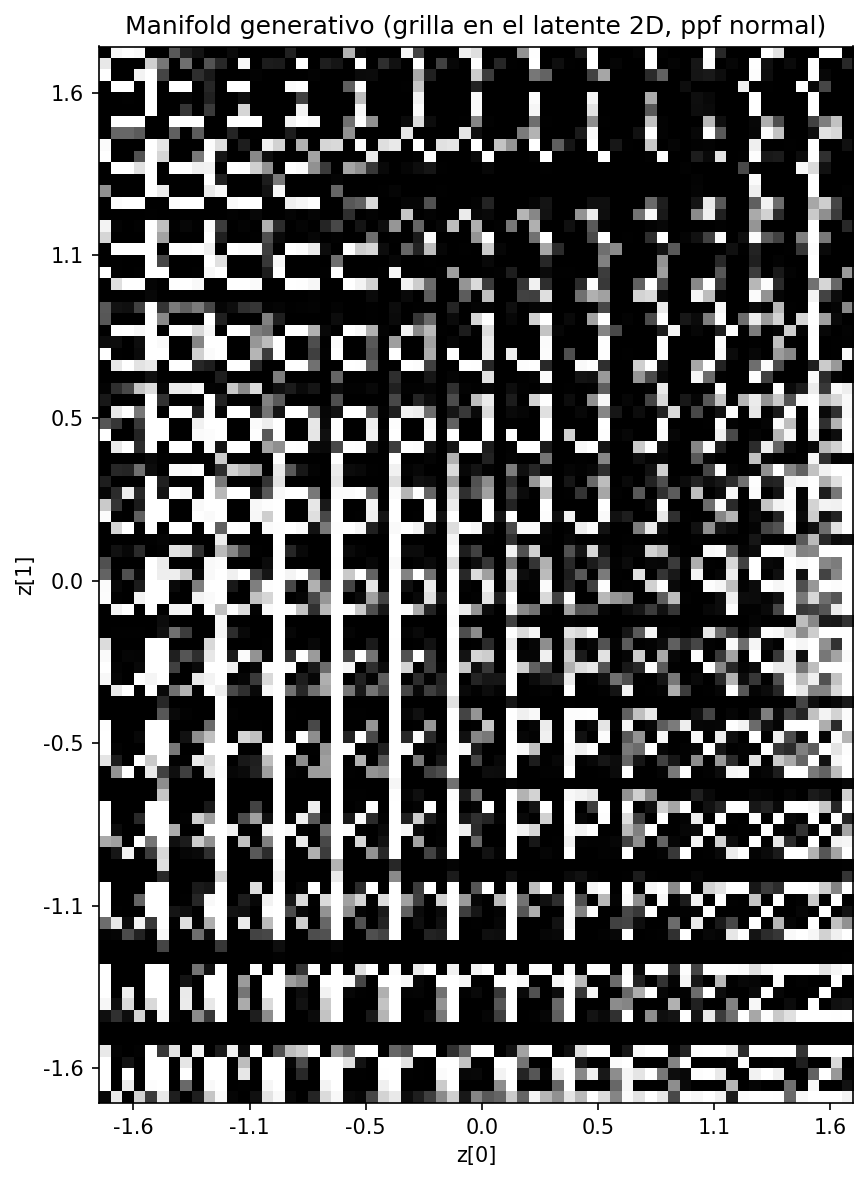
\includegraphics[height=0.78\textheight]{letters_vae_manifold.png}\\
      {\scriptsize Manifold 2D: grilla de $z$ decodificada (se ven \texttt{P,o,d,k,z}\dots).}
    \end{column}
  \end{columns}
\end{frame}

\begin{frame}{AE vs VAE: ¿que compra el termino KL?}
  \centering
  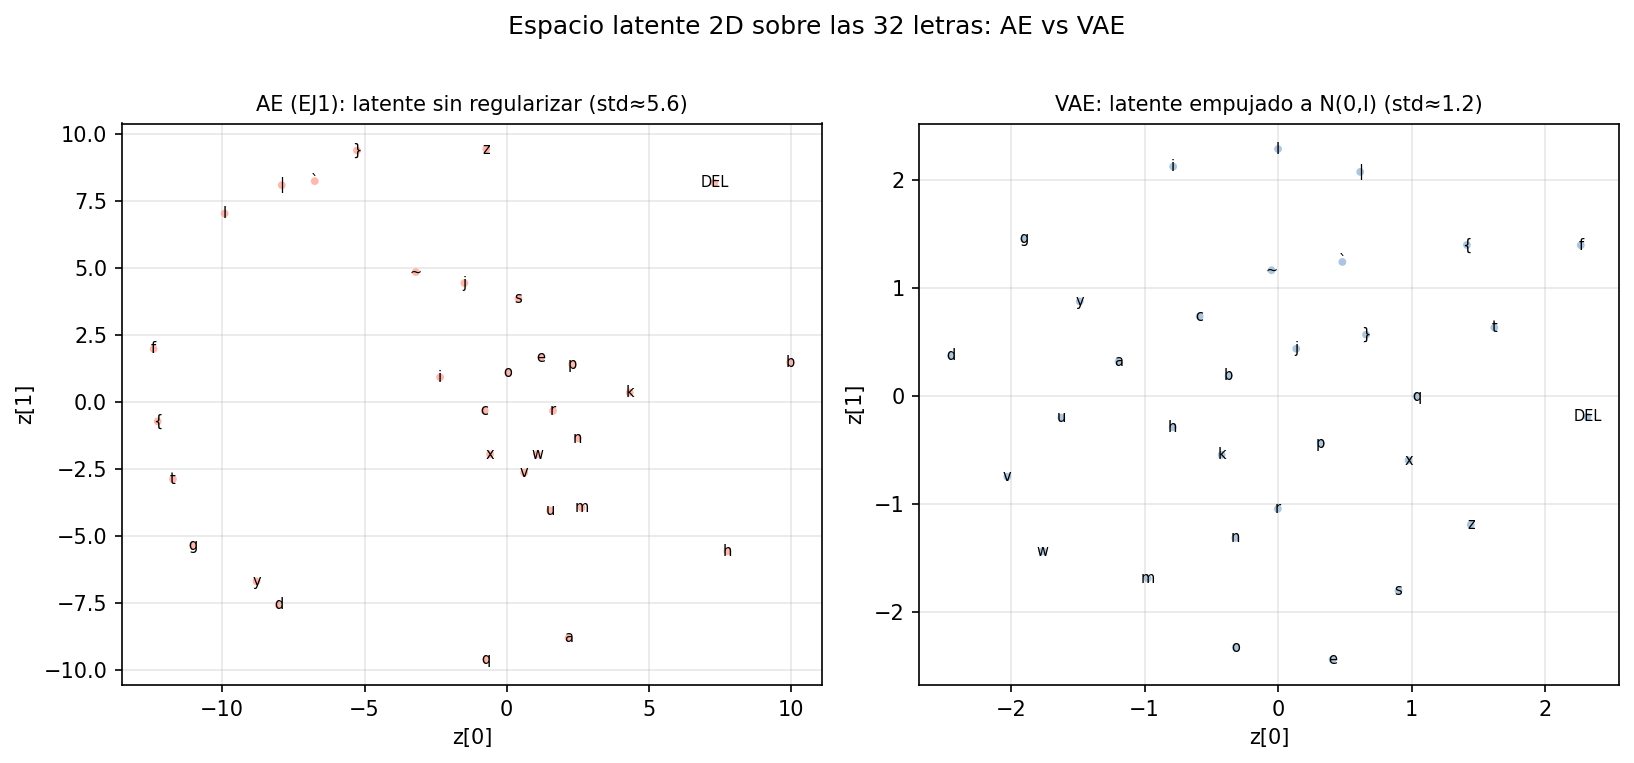
\includegraphics[width=0.92\linewidth]{letters_ae_vs_vae_scatter.png}
  \vfill
  {\footnotesize Mismos datos, latente 2D. El \textbf{AE} desparrama los codigos
   sin estructura (std $\approx 5.6$, rango $\pm 13$); el \textbf{VAE} los empuja
   a $\mathcal{N}(0,I)$ (std $\approx 1.2$, centrado en 0). Por eso \emph{muestrear
   del prior} funciona en el VAE y no en el AE.}
\end{frame}

\begin{frame}{AE vs VAE: muestreo del prior e interpolacion}
  \begin{columns}
    \begin{column}{0.5\textwidth}
      \centering
      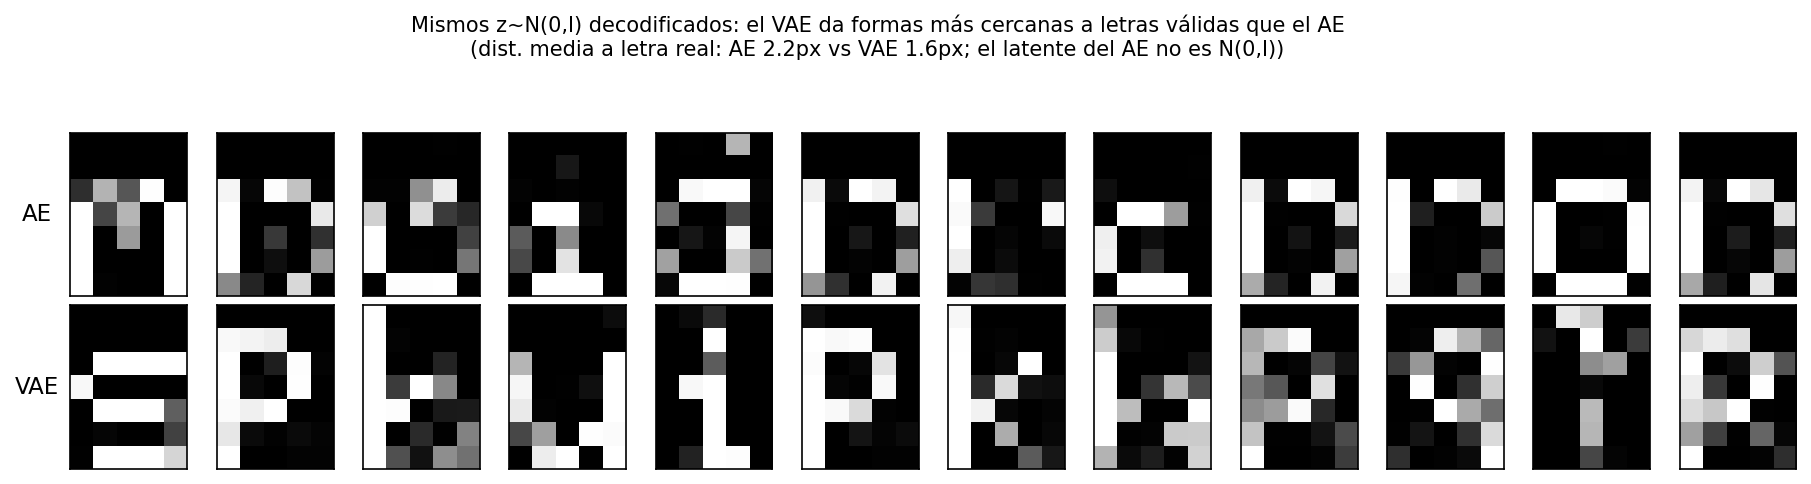
\includegraphics[width=\linewidth]{letters_ae_vs_vae_samples.png}\\
      {\scriptsize Mismos $z\sim\mathcal{N}(0,I)$ decodificados. Dist.\ media a
       letra real: \textbf{VAE 1.6 px} vs AE 2.2 px.}
    \end{column}
    \begin{column}{0.5\textwidth}
      \centering
      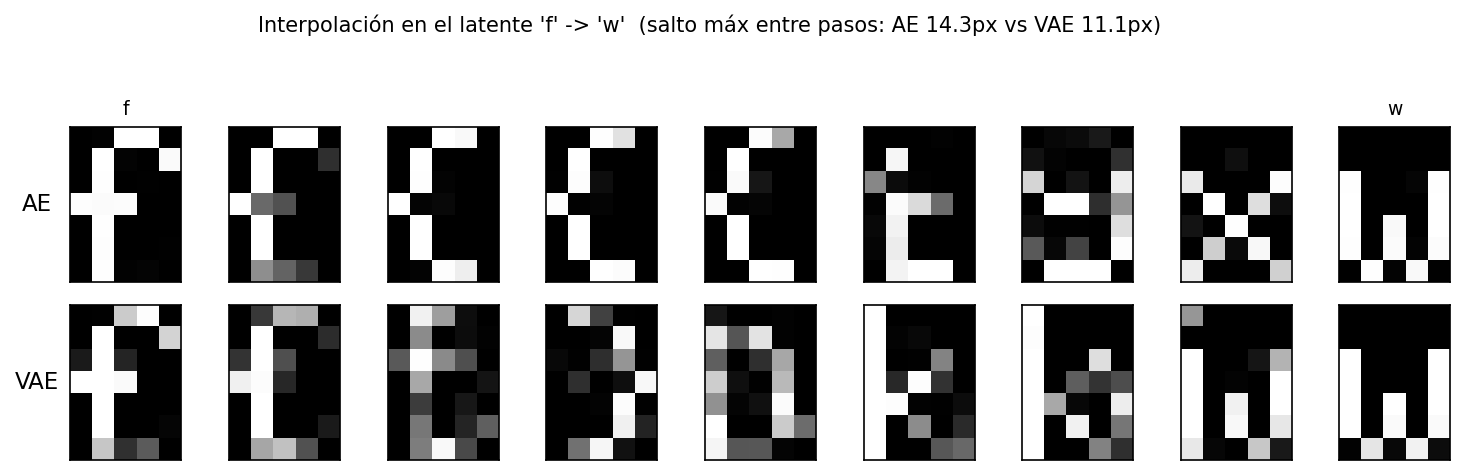
\includegraphics[width=\linewidth]{letters_ae_vs_vae_interp.png}\\
      {\scriptsize Interpolacion \texttt{f}$\to$\texttt{w}. Salto maximo entre
       pasos: \textbf{VAE 11.1 px} vs AE 14.3 px (mas gradual).}
    \end{column}
  \end{columns}
  \vfill
  {\footnotesize Con solo 32 puntos el efecto es \emph{modesto} pero consistente:
   el latente del VAE es mas usable como espacio generativo. En emojis/MNIST
   (mas datos) la diferencia es mayor.}
\end{frame}

% ===========================================================================
\section{B --- Unidades activas (posterior collapse)}

\begin{frame}{¿Por que satura el latente? Unidades activas}
  \begin{columns}
    \begin{column}{0.42\textwidth}
      \begin{itemize}
        \item KL \emph{por dimension}:
              \[ \mathrm{KL}_j = \mathbb{E}_x\!\left[-\tfrac12(1+\log\sigma_j^2-\mu_j^2-\sigma_j^2)\right] \]
        \item Si la dim $j$ \textbf{colapsa} al prior $\Rightarrow \mathrm{KL}_j\approx 0$
              (no transporta informacion).
        \item ``Activa'' $=\mathrm{KL}_j > 0{,}01$.
        \item En MNIST, con latente 32 o 64 \textbf{la mayoria de las dims
              colapsan} (rojo).
      \end{itemize}
    \end{column}
    \begin{column}{0.58\textwidth}
      \centering
      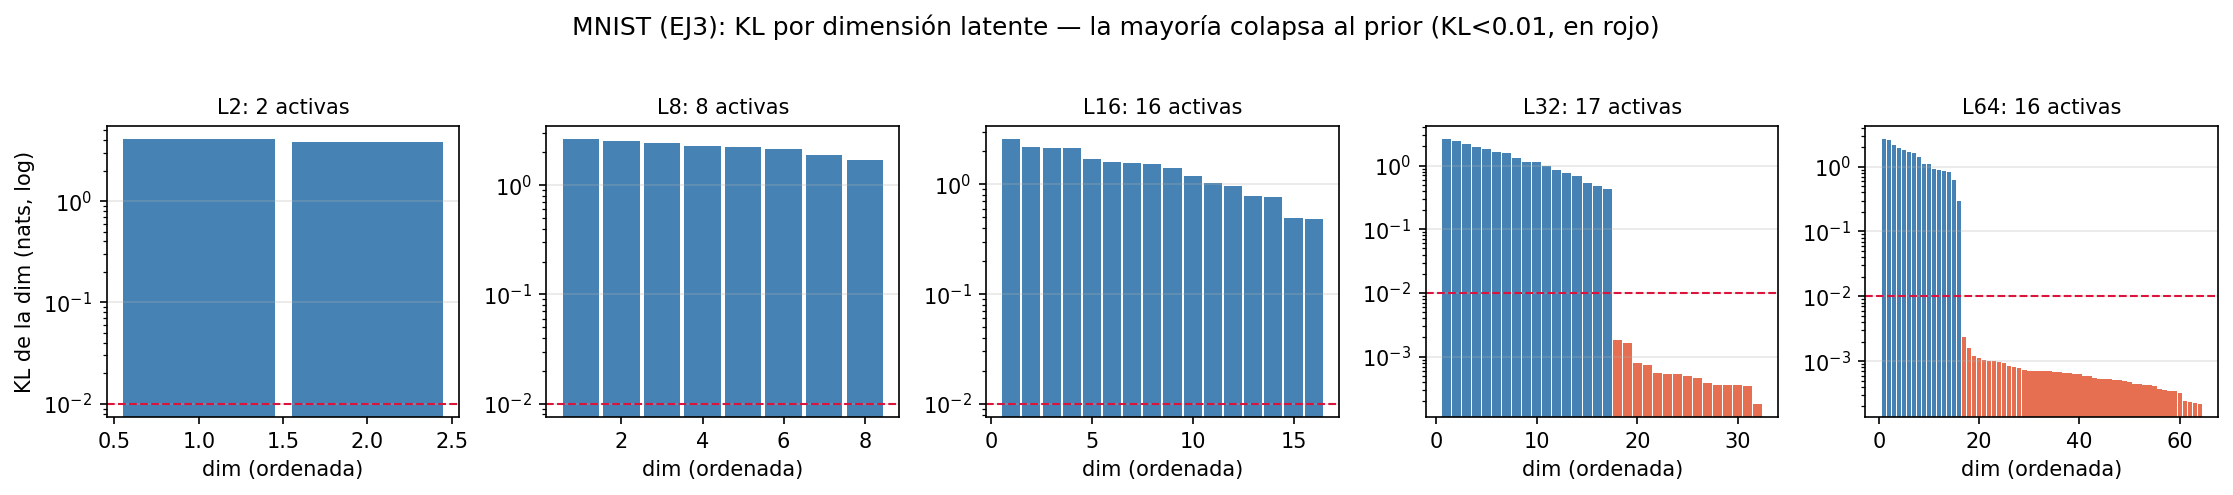
\includegraphics[width=\linewidth]{active_units_kl_spectrum.png}\\
      {\scriptsize MNIST (EJ3): KL por dimension (ordenada). En rojo, las dims
       colapsadas ($\mathrm{KL}<0{,}01$).}
    \end{column}
  \end{columns}
\end{frame}

\begin{frame}{El VAE usa un numero limitado de dimensiones}
  \begin{columns}
    \begin{column}{0.54\textwidth}
      \centering
      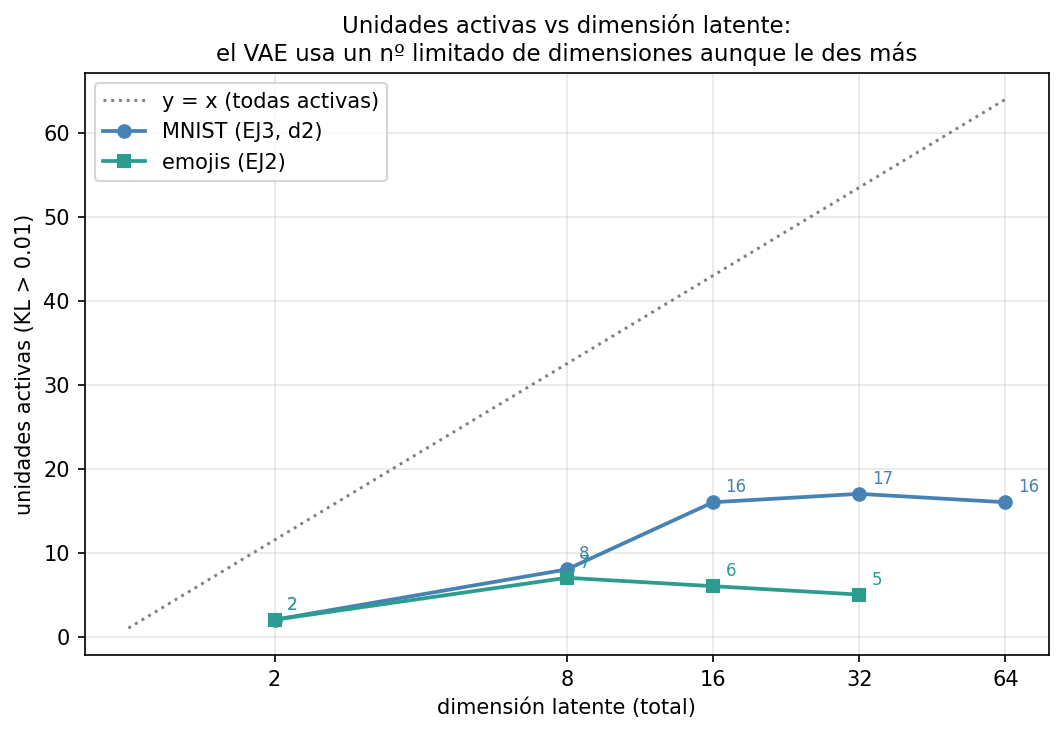
\includegraphics[width=\linewidth]{active_units_vs_latent.png}
    \end{column}
    \begin{column}{0.46\textwidth}
      \centering
      {\footnotesize MNIST (EJ3, arquitectura d2):}\\[2pt]
      \begin{tabular}{rcc}
        \toprule
        latente & activas & KL total \\
        \midrule
        2  & 2/2   & 7{,}9 \\
        8  & 8/8   & 17{,}8 \\
        16 & 16/16 & 22{,}5 \\
        32 & \textbf{17}/32 & 22{,}5 \\
        64 & \textbf{16}/64 & 22{,}5 \\
        \bottomrule
      \end{tabular}
      \vfill
      {\footnotesize \textbf{El mecanismo de la saturacion:} aunque demos 32 o
       64 dimensiones, el VAE solo activa $\sim$16--17; el KL total se clava en
       $\approx 22{,}5$. Por eso la calidad no mejora pasando de 16--32.}
    \end{column}
  \end{columns}
\end{frame}

% ===========================================================================
\section{D --- Generalizacion (train/test)}

\begin{frame}{¿El VAE de emojis memoriza o generaliza?}
  \begin{columns}
    \begin{column}{0.56\textwidth}
      \centering
      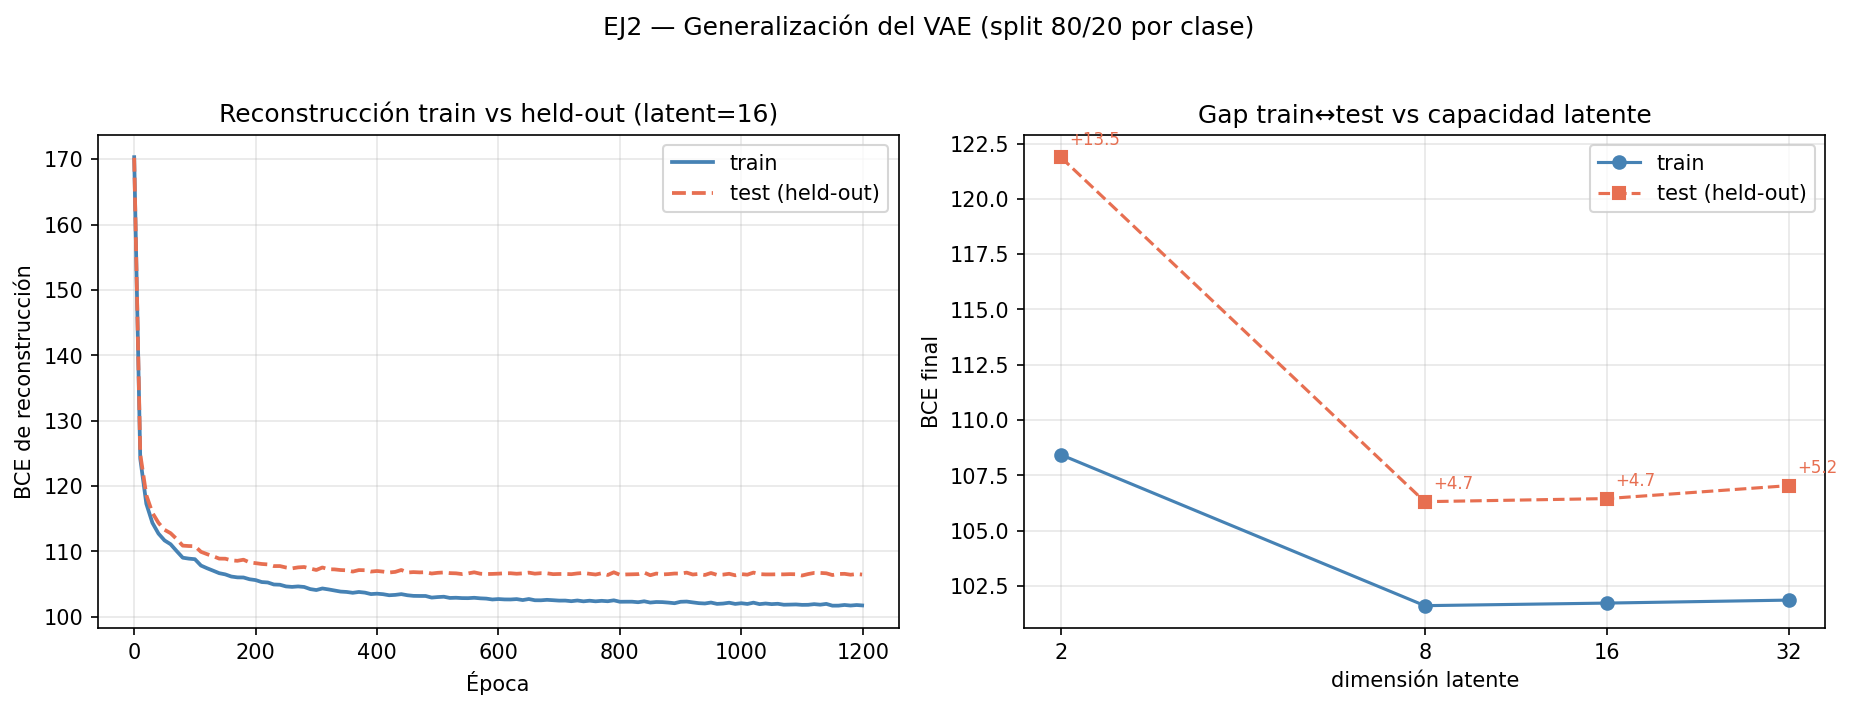
\includegraphics[width=\linewidth]{generalization_curves.png}
    \end{column}
    \begin{column}{0.44\textwidth}
      {\footnotesize
      \begin{itemize}
        \item Split \textbf{80/20} estratificado por clase (held-out de
              variantes nunca vistas); disciplina del TP3, ausente en EJ2.
        \item El test \textbf{sigue al train} (no sube): \textbf{generaliza},
              no memoriza. Gap chico ($\sim\!+5$ BCE).
        \item El gap \textbf{no crece} con la dim latente (8/16/32 dan $\sim\!+5$;
              latente 2 \emph{underfitea}, $+13$).
        \item \textcolor{green!50!black}{Conecta con B:} el posterior collapse
              limita la capacidad \emph{efectiva} ($\sim$5--7 dims activas), asi
              que mas latente \emph{no} agrega sobreajuste.
      \end{itemize}}
      \centering
      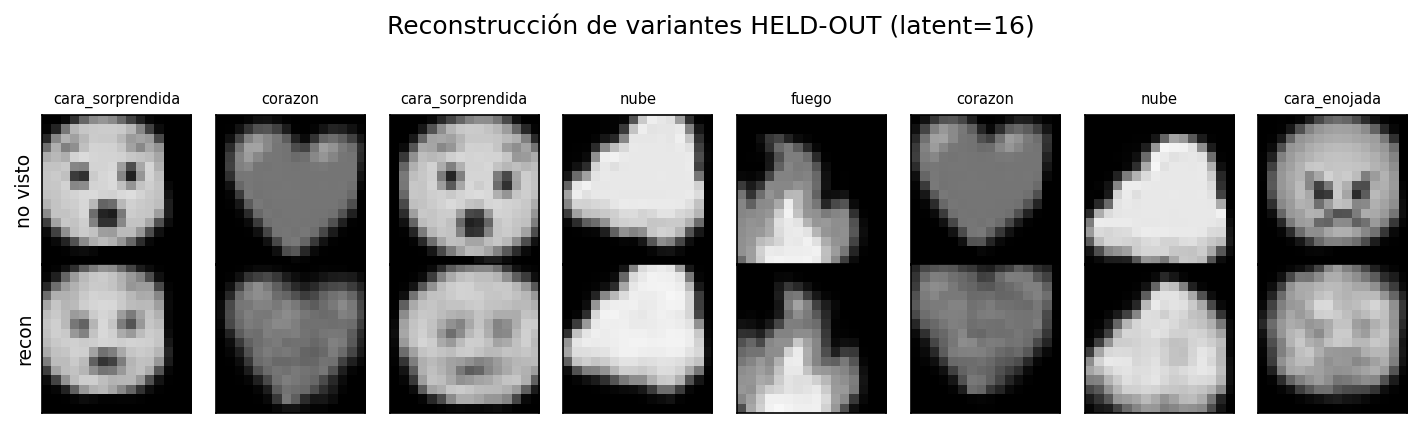
\includegraphics[width=0.82\linewidth]{generalization_heldout.png}
    \end{column}
  \end{columns}
\end{frame}

% ===========================================================================
\section{E --- MSE vs BCE}

\begin{frame}{Perdida de reconstruccion: MSE vs BCE}
  \centering
  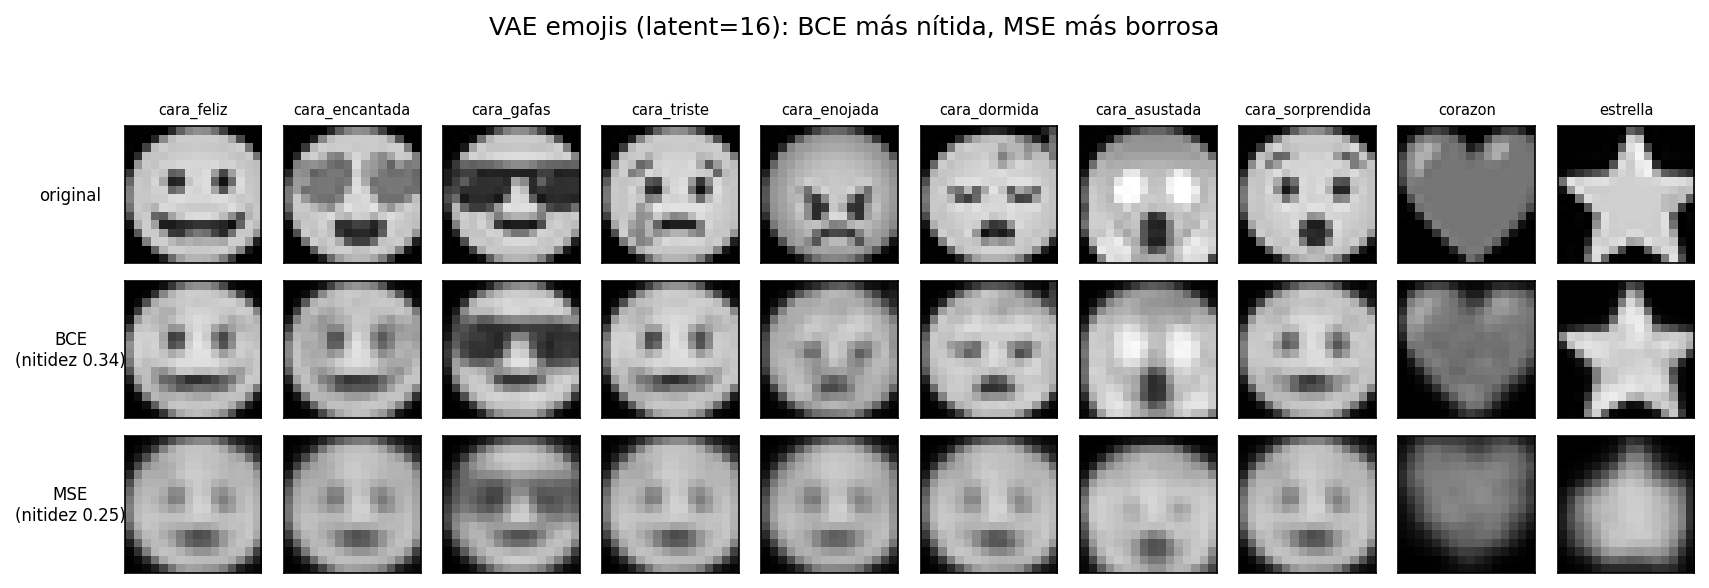
\includegraphics[width=0.96\linewidth]{recon_loss_mse_vs_bce.png}
  \vfill
  {\footnotesize Dos VAE identicos salvo la \texttt{recon\_loss} (misma salida
   logistica, latente 16, 600 ep). \textbf{BCE} es mas nitida (nitidez $0{,}34$
   vs $0{,}25$) y ademas reconstruye mejor \emph{aun medido en MSE} ($1{,}4$ vs
   $5{,}2$): MSE${+}$sigmoide tiene gradiente que se \textbf{desvanece} cerca de
   $0/1$, asi que entrena peor a igual presupuesto.}
\end{frame}

% ===========================================================================
\section{Resumen}

\begin{frame}{Resumen y recomendacion}
  \begin{itemize}
    \item \textbf{B (posterior collapse)} --- el mas fuerte: explica
          \emph{cuantitativamente} por que el latente satura (solo $\sim$16
          dims activas de 64). \textcolor{green!50!black}{Recomendado integrar.}
    \item \textbf{A (VAE sobre letras)} --- buen puente narrativo AE$\to$VAE
          sobre datos ya conocidos; el scatter AE vs VAE es muy claro.
    \item \textbf{E (MSE vs BCE)} --- barato y visual; justifica la eleccion de
          BCE de la principal.
    \item \textbf{D (train/test)} --- aporta rigor (el VAE \emph{generaliza};
          gap acotado por el posterior collapse de B, no crece con el latente).
  \end{itemize}
  \vfill
  {\footnotesize Todos los datos crudos quedan en \texttt{extra/results/} (\texttt{*.csv},
   \texttt{*.npz}) para regraficar sin re-entrenar.}
\end{frame}

\end{document}
